\documentclass[10pt]{article}
\usepackage[T1]{fontenc}
\usepackage{lmodern,microtype,xcolor,booktabs,array,enumitem,ragged2e,caption,standalone,tikz,pgfplots}
\usepgfplotslibrary{groupplots}
\usetikzlibrary{arrows.meta,positioning}
\usepackage[letterpaper,margin=0.49in,top=0.43in,bottom=0.40in]{geometry}
\definecolor{briefblue}{HTML}{005B96}
\definecolor{briefcyan}{HTML}{EAF4F8}
\definecolor{briefgold}{HTML}{D99000}
\definecolor{briefgreen}{HTML}{17855B}
\definecolor{briefgray}{HTML}{4D5963}
\definecolor{atlas0}{HTML}{0072B2}
\definecolor{atlas1}{HTML}{E69F00}
\definecolor{atlas2}{HTML}{009E73}
\definecolor{atlas3}{HTML}{CC79A7}
\definecolor{atlas4}{HTML}{D55E00}
\definecolor{atlas5}{HTML}{56B4E9}
\definecolor{atlas6}{HTML}{000000}
\definecolor{atlas7}{HTML}{6A3D9A}
\definecolor{atlas8}{HTML}{A6CEE3}
\definecolor{atlas9}{HTML}{B2DF8A}
\definecolor{supervisor0}{HTML}{0072B2}
\definecolor{supervisor1}{HTML}{E69F00}
\definecolor{supervisor2}{HTML}{009E73}
\definecolor{supervisor3}{HTML}{CC79A7}
\definecolor{supervisor4}{HTML}{D55E00}
\definecolor{supervisor5}{HTML}{56B4E9}
\definecolor{supervisor6}{HTML}{000000}
\definecolor{supervisor7}{HTML}{6A3D9A}
\definecolor{supervisor8}{HTML}{A6CEE3}
\definecolor{supervisor9}{HTML}{B2DF8A}
\pgfplotsset{compat=1.18}
\pdfinfoomitdate=1
\pdftrailerid{}
\pdfsuppressptexinfo=-1
\setlength{\parindent}{0pt}
\setlength{\parskip}{2pt}
\setlist[itemize]{leftmargin=1.15em,itemsep=0.5pt,topsep=1pt,parsep=0pt}
\setlist[enumerate]{leftmargin=1.3em,itemsep=0.5pt,topsep=1pt,parsep=0pt}
\captionsetup{font=footnotesize,labelfont=bf,skip=2pt}
\pagestyle{empty}
\newcommand{\sectionbar}[1]{\vspace{2pt}{\color{briefblue}\rule{\linewidth}{0.8pt}}\vspace{-7pt}\section*{\color{briefblue}#1}\vspace{-5pt}}
\newcommand{\keybox}[1]{\begin{center}\begin{tikzpicture}\node[rounded corners=2pt,fill=briefcyan,draw=briefblue!55,inner xsep=7pt,inner ysep=5pt,text width=.965\linewidth,align=left,font=\small]{#1};\end{tikzpicture}\end{center}}
\begin{document}
\fontsize{8.75}{10.35}\selectfont
\begin{minipage}[t]{.72\linewidth}
{\fontsize{16}{18}\selectfont\bfseries\color{briefblue}ATLAS field-trial SERS dataset}\par
{\fontsize{11}{13}\selectfont\bfseries Construction, preliminary evidence, and research direction}
\end{minipage}\hfill
\begin{minipage}[t]{.25\linewidth}\raggedleft\color{briefgray}Supervisor discussion brief\\25 August 2026\end{minipage}

\keybox{A source-reversible audit reduced \textbf{721 explicitly named SERS observations} to \textbf{598 unique, numeric, chemically attributable spectra} from \textbf{69 physical samples}. Repeated multi-instrument measurements make the dataset suitable for chemical identification under acquisition shift; they do not establish a clean-spectrum reference or causal nuisance separation.}

\sectionbar{1. Dataset construction}
\begin{center}
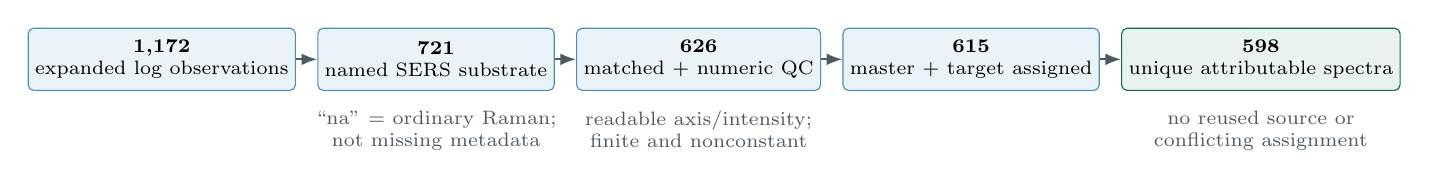
\begin{tikzpicture}[node distance=2.7mm,
stage/.style={rounded corners=2pt,draw=briefblue!70,fill=briefcyan,minimum width=2.95cm,minimum height=.79cm,align=center,inner sep=2.5pt,font=\scriptsize},
last/.style={stage,draw=briefgreen!80!black,fill=briefgreen!10},arrow/.style={-{Latex[length=2mm]},line width=.7pt,draw=briefgray}]
\node[stage](a){\textbf{1,172}\\expanded log observations};
\node[stage,right=of a](b){\textbf{721}\\named SERS substrate};
\node[stage,right=of b](c){\textbf{626}\\matched + numeric QC};
\node[stage,right=of c](d){\textbf{615}\\master + target assigned};
\node[last,right=of d](e){\textbf{598}\\unique attributable spectra};
\draw[arrow](a)--(b);\draw[arrow](b)--(c);\draw[arrow](c)--(d);\draw[arrow](d)--(e);
\node[font=\scriptsize,align=center,text=briefgray,below=1.3mm of b]{``na'' = ordinary Raman;\\not missing metadata};
\node[font=\scriptsize,align=center,text=briefgray,below=1.3mm of c]{readable axis/intensity;\\finite and nonconstant};
\node[font=\scriptsize,align=center,text=briefgray,below=1.3mm of e]{no reused source or\\conflicting assignment};
\end{tikzpicture}
\end{center}

\begin{minipage}[t]{.485\linewidth}
\textbf{Resulting analysis population}
\begin{itemize}
\item 598 spectra, but only \textbf{69 independent physical samples}.
\item 10 instruments, 4 SERS sensor families, 3 stations, and 7 recorded labels.
\item Repeated views remain linked by one physical-master identifier.
\item The 500-spectrum notes-clear and 575-spectrum Mira-1-excluded tiers are retained for sensitivity analysis.
\end{itemize}
\end{minipage}\hfill
\begin{minipage}[t]{.495\linewidth}
\textbf{Primary spectral representation}
\begin{itemize}
\item Common measured support: \textbf{400--1,800 cm$^{-1}$}; no low-shift extrapolation.
\item Interpolation at 1 cm$^{-1}$ gives \textbf{1,401 ordered coordinates}.
\item Each spectrum is independently min--max scaled to $[0,1]$.
\item SG and arPLS are retained as candidates; minimal scaling is the reference, not a claimed optimum.
\end{itemize}
\end{minipage}

\begin{center}
\resizebox{.84\linewidth}{!}{\includestandalone[mode=tex]{../figures/supervisor_update/tikz/F05_instrument_spectra}}
\captionof{figure}{Instrument median spectra before and after row-wise scaling. Scaling removes the absolute intensity range but preserves visible acquisition-dependent background and shape differences.}
\end{center}
\vfill
{\scriptsize\color{briefgray}\textbf{Interpretation boundary:} these instrument summaries do not identify which differences are chemical, instrumental, sensor-related, or sample-specific.}

\newpage
\sectionbar{2. Preliminary evidence and research direction}
\begin{minipage}[t]{.47\linewidth}
\textbf{Acquisition dominates the raw geometry.} Raw channel-standardized PCA assigns \textbf{93.68\%} of variance to PC1. Row-wise min--max scaling reduces PC1 to \textbf{42.68\%}; the remaining clusters are still more associated with instrument than chemistry.
\end{minipage}\hfill
\begin{minipage}[t]{.51\linewidth}
\textbf{Chemical information remains measurable.} Combining repeated measurements within each physical sample increases chemical cluster association to \textbf{0.668}, although station association remains \textbf{0.585}. Chemistry and acquisition context are therefore not fully separated.
\end{minipage}

\begin{center}
\resizebox{.64\linewidth}{!}{\includestandalone[mode=tex]{../figures/supervisor_update/tikz/S01_pca_recolored}}
\captionof{figure}{The same min--max PCA coordinates colored by instrument and chemical. Instrument labels produce clearer groups; PCA is descriptive and is not classification performance.}
\end{center}

\begin{minipage}[t]{.43\linewidth}
\begin{center}
\resizebox{.72\linewidth}{!}{\includestandalone[mode=tex]{../figures/supervisor_update/tikz/S02_cluster_association_scatter}}
\captionof{figure}{Cluster association under candidate representations. Below the diagonal indicates stronger instrument association.}
\end{center}
\end{minipage}\hfill
\begin{minipage}[t]{.555\linewidth}
\textbf{Preprocessing trade-off.} Min--max cluster association is \textbf{0.482} with instrument and \textbf{0.287} with chemical identity. arPLS lowers these values to \textbf{0.094} and \textbf{0.065}. Reduced instrument association alone therefore does not show that chemistry was preserved.

\textbf{Questions supported by the data}
\begin{enumerate}
\item Can supported chemicals be identified on an unseen instrument and unseen physical samples?
\item Do universal or source-selected preprocessing rules improve transfer without damaging peaks?
\item Do compact or acquisition-aware deep models improve on tuned classical methods?
\item What is gained from calibration samples, and can unfamiliar cases be flagged?
\end{enumerate}

\textbf{Why these questions fit.} Repeated cross-instrument views expose acquisition shift while retaining physical-sample identity. The 69-master sample size favours controlled classical models and compact neural networks.
\end{minipage}

\vspace{3pt}
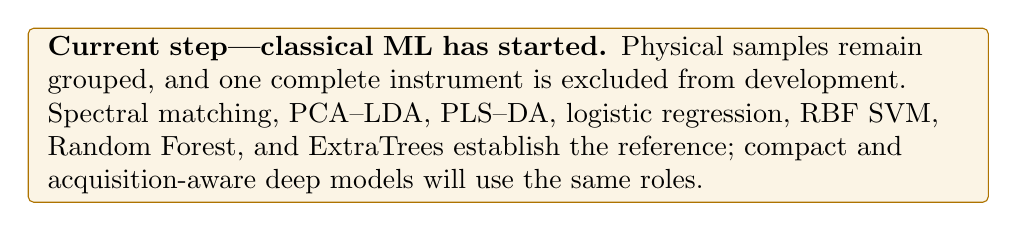
\begin{tikzpicture}
\node[rounded corners=2pt,draw=briefgold!80!black,fill=briefgold!10,inner xsep=7pt,inner ysep=3pt,text width=.965\linewidth,align=left]{\textbf{Current step---classical ML has started.} Physical samples remain grouped, and one complete instrument is excluded from development. Spectral matching, PCA--LDA, PLS--DA, logistic regression, RBF SVM, Random Forest, and ExtraTrees establish the reference; compact and acquisition-aware deep models will use the same roles.};
\end{tikzpicture}

{\scriptsize\color{briefgray}\textbf{Boundary:} no universally best preprocessing, clean-spectrum recovery, causal disentanglement, or arbitrary-domain generalization is claimed.}
\end{document}
